\documentclass[11pt,a4paper]{article}
\usepackage[a4paper,left=1.5in,right=1in,top=1in,bottom=1in]{geometry}
\usepackage{setspace}
\singlespacing
\usepackage{pgfgantt}
\usepackage{float}
\usepackage[utf8]{inputenc}
\usepackage[T1]{fontenc}
\usepackage{amsmath,amssymb}
\usepackage{tikz}
\usetikzlibrary{arrows.meta,positioning,calc}
\usepackage{booktabs}
\usepackage{tabularx}
\usepackage{enumitem}
\usepackage{xcolor}
\usepackage{filecontents}
\usepackage[hidelinks]{hyperref}

% ---------------------------------------------------------------------
% EMBEDDED BIBLIOGRAPHY (keeps the submission to ONE file).
% This block writes out refs.bib at compile time -- do not create or
% edit refs.bib directly; edit this block instead. Mirror these records
% in your Zotero collection; Zotero exports BibTeX directly, so this
% block should just be pasted-in Zotero output going forward.
% Entries marked VERIFY must be checked against the actual source
% before the final submission.
% ---------------------------------------------------------------------
\begin{filecontents*}[overwrite]{refs.bib}
@misc{chipsandcheese_graviton4,
  author       = {Lam, Chester},
  title        = {Arm's {Neoverse} {V2}, in {AWS}'s {Graviton}~4},
  year         = {2024},
  howpublished = {Chips and Cheese,
                  \url{https://chipsandcheese.com/p/arms-neoverse-v2-in-awss-graviton-4}}
}
@misc{chipsandcheese_zen5,
  author       = {{Chips and Cheese}},
  title        = {Disabling {Zen}~5's Op Cache and Exploring Its
                  Clustered Decoder},
  year         = {2025},
  howpublished = {\url{https://chipsandcheese.com/p/disabling-zen-5s-op-cache-and-exploring}}
}
@misc{hothardware_turin,
  author       = {{HotHardware}},
  title        = {{AMD} {EPYC} 9005 5th-Gen {Turin} {CPUs} Arrive With
                  Up to 192 Cores},
  year         = {2024},
  howpublished = {\url{https://hothardware.com/news/amd-epyc-5th-gen-launch}}
}
@misc{hothardware_xeon6,
  author       = {{HotHardware}},
  title        = {Intel Launches {Xeon} 6900{P}, 128 {P}-Core
                  {Granite} {Rapids}},
  year         = {2024},
  howpublished = {\url{https://hothardware.com/reviews/intel-xeon-6-6900p-with-p-cores-launch}}
}
@misc{awsgravitonguide,
  author       = {{Amazon Web Services}},
  title        = {{AWS Graviton Getting Started and Technical Guide},
  year         = {2026},
  howpublished = {\url{https://github.com/aws/aws-graviton-getting-started}},
  note         = {Accessed: 24 August 2026}
}

@misc{amdepyc,
  author       = {{Advanced Micro Devices}},
  title        = {{AMD} {EPYC} 9005 Series Processor Architecture Overview},
  year         = {2024},
  note         = {Document 58462, Rev. 1.0}
}

@misc{intelxeon,
  author       = {{Intel Corporation}},
  title        = {{Intel} {Xeon} 6 Processors: Architecture and
                  Performance Documentation},
  year         = {2025},
  note         = {Accessed: 24 August 2026}
}

@misc{phoronix2022,
  author       = {Larabel, Michael},
  title        = {Benchmarking {Amazon} {Graviton} Against {AMD} {EPYC}
                  and {Intel} {Xeon}},
  howpublished = {Phoronix},
  year         = {2022},
  note         = {Earlier-generation same-cloud benchmark; VERIFY exact
                  article details before final submission}
}

@article{lawenda2025,
  author  = {Lawenda, Marcin and Szustak, {\L}ukasz and
             K{\"o}rnyei, L{\'a}szl{\'o} and
             Galeazzo, Flavio Cesar Cunha and Bratek, Pawe{\l}},
  title   = {Evaluating the Impact of the {L3} Cache Size of {AMD} {EPYC}
             {CPUs} on the Performance of {CFD} Applications},
  journal = {arXiv preprint arXiv:2505.17934},
  year    = {2025},
  doi     = {10.48550/arXiv.2505.17934},
  url     = {https://arxiv.org/abs/2505.17934}
}

@article{hofmann2015,
  author  = {Hofmann, Johannes and Eitzinger, Jan and Fey, Dietmar},
  title   = {Execution-Cache-Memory Performance Model:
             Introduction and Validation},
  journal = {arXiv preprint arXiv:1509.03118},
  year    = {2015},
  url     = {https://arxiv.org/abs/1509.03118}
}

@misc{awsperftesting,
  author       = {{Amazon Web Services}},
  title        = {{AWS Graviton Performance Testing:
                  Tips for Independent Software Vendors}},
  year         = {2021},
  month        = sep,
  day          = {15},
  howpublished = {AWS Whitepaper},
  url          = {https://docs.aws.amazon.com/whitepapers/latest/aws-graviton-performance-testing/aws-graviton-performance-testing.html},
  note         = {Accessed: 24 August 2026}
}

@misc{phoronix2025,
  author       = {Larabel, Michael},
  title        = {{AMD} {EPYC} {Turin} vs. {Intel} {Xeon} 6 {Granite}
                  {Rapids} vs. {Graviton4} Benchmarks With {AWS} M8
                  Instances},
  howpublished = {Phoronix},
  year         = {2025},
  month        = oct,
  day          = {24},
  url          = {https://www.phoronix.com/review/aws-m8a-m8g-m8i-benchmarks},
  note         = {Accessed: 24 August 2026}
}
@misc{aws2021gravitontesting,
  author       = {{Amazon Web Services}},
  title        = {{AWS Graviton Performance Testing:
                  Tips for Independent Software Vendors}},
  year         = {2021},
  month        = sep,
  day          = {15},
  howpublished = {AWS Whitepaper},
  url          = {https://docs.aws.amazon.com/whitepapers/latest/aws-graviton-performance-testing/aws-graviton-performance-testing.html},
  note         = {Accessed: 24 August 2026}
}
@article{hofmann2015ecm,
  author  = {Hofmann, Johannes and Eitzinger, Jan and Fey, Dietmar},
  title   = {Execution-Cache-Memory Performance Model:
             Introduction and Validation},
  journal = {arXiv preprint arXiv:1509.03118},
  year    = {2015},
  url     = {https://arxiv.org/abs/1509.03118}
}
@article{lawenda2025epyc,
  author  = {Lawenda, Marcin and Szustak, {\L}ukasz and
             K{\"o}rnyei, L{\'a}szl{\'o} and
             Galeazzo, Flavio Cesar Cunha and Bratek, Pawe{\l}},
  title   = {Evaluating the Impact of the {L3} Cache Size of {AMD} {EPYC}
             {CPUs} on the Performance of {CFD} Applications},
  journal = {arXiv preprint arXiv:2505.17934},
  year    = {2025},
  doi     = {10.48550/arXiv.2505.17934},
  url     = {https://arxiv.org/abs/2505.17934}
}
@misc{larabel2025m8,
  author       = {Larabel, Michael},
  title        = {{AMD} {EPYC} {Turin} vs. {Intel} {Xeon} 6 {Granite}
                  {Rapids} vs. {Graviton4} Benchmarks With {AWS} M8
                  Instances},
  howpublished = {Phoronix},
  year         = {2025},
  month        = oct,
  day          = {24},
  url          = {https://www.phoronix.com/review/aws-m8a-m8g-m8i-benchmarks},
  note         = {Accessed: 24 August 2026}
}
@misc{awsgraviton,
  author       = {{Amazon Web Services}},
  title        = {{AWS Graviton Getting Started and Technical Guide}},
  year         = {2026},
  howpublished = {\url{https://github.com/aws/aws-graviton-getting-started}},
  note         = {Accessed: 24 August 2026}
}
@book{sarangi,
  author    = {Sarangi, Smruti R.},
  title     = {Computer Organisation and Architecture},
  publisher = {McGraw Hill Education},
  year      = {2015},
  note      = {Prescribed textbook. Online: https://srsarangi.github.io/archbook/archbook.pdf}
}
@book{hennessy,
  author    = {Hennessy, John L. and Patterson, David A.},
  title     = {Computer Architecture: A Quantitative Approach},
  edition   = {6th},
  publisher = {Morgan Kaufmann},
  year      = {2019}
}
@inproceedings{velten2022,
  author    = {Velten, Markus and Sch{\"o}ne, Robert and Ilsche, Thomas
               and Hackenberg, Daniel},
  title     = {Memory Performance of {AMD} {EPYC} {Rome} and {Intel}
               {Cascade} {Lake} {SP} Server Processors},
  booktitle = {Proceedings of the 2022 ACM/SPEC International Conference
               on Performance Engineering (ICPE)},
  year      = {2022},
  doi       = {10.1145/3489525.3511689},
  note      = {Preprint: arXiv:2204.03290}
}
@book{nagarajan2020,
  author    = {Nagarajan, Vijay and Sorin, Daniel J. and Hill, Mark D.
               and Wood, David A.},
  title     = {A Primer on Memory Consistency and Cache Coherence},
  edition   = {2nd},
  publisher = {Morgan and Claypool},
  year      = {2020}
}
@misc{awsgraviton,
  author       = {{Amazon Web Services}},
  title        = {{AWS} {Graviton} Getting Started and Technical Guide},
  year         = {2026},
  howpublished = {\url{https://github.com/aws/aws-graviton-getting-started}},
  note         = {VERIFY exact document title and access date}
}
@misc{amdepyc,
  author       = {{Advanced Micro Devices}},
  title        = {{AMD} {EPYC} 9005 Series Processor Architecture Overview},
  year         = {2024},
  note         = {VERIFY document number and revision}
}
@misc{intelxeon,
  author       = {{Intel Corporation}},
  title        = {{Intel} {Xeon} 6 Processors: Product Brief and
                  Architecture Documentation},
  year         = {2025},
  note         = {VERIFY document number and revision}
}
@misc{phoronix2025,
  author       = {Larabel, Michael},
  title        = {{AMD} {EPYC} {Turin} vs. {Intel} {Xeon} 6 {Granite} {Rapids}
                  vs. {Graviton4} Benchmarks With {AWS} M8 Instances},
  howpublished = {Phoronix},
  year         = {2025},
  note         = {Same-cloud comparative benchmark data. VERIFY date}
}
\end{filecontents*}

% ---------------------------------------------------------------------
\newcommand{\fillin}[1]{\textcolor{red}{\textbf{[FILL IN: #1]}}}

\title{\textbf{AWS Graviton vs.\ AMD EPYC vs.\ Intel Xeon:\\
A Comparative Architecture Analysis of\\ Modern Server Processors}}

\author{
  {Animesh Sachan, 2024EE10935} \\
  {Adil Khan, 2024MT10256} \\[6pt]
  Department of Electrical Engineering \\
  Indian Institute of Technology Delhi \\[4pt]
  ELL305 Computer Architecture --- Term Paper --- Draft 1 (v0.1)
}
\date{24 August 2026}
\begin{document}
\maketitle

\begin{abstract}
\noindent
This document reports the progress made on the term paper titled \emph{AWS Graviton vs.\ AMD
EPYC vs.\ Intel Xeon: A Comparative Architecture Analysis of Modern Server Processors} as of
24 August 2026. Per the instructions for Draft~1, this document is a \textbf{progress report}
--- the ``Background Preparations'' expected at this stage --- and not a preliminary version of
the final $\sim$150-page term paper.

The chosen topic undertakes a comparative architectural study of three families of modern
data-centre server processors: Amazon Web Services' custom Arm-based Graviton processors,
AMD's x86-64 EPYC processors (Zen microarchitecture family), and Intel's x86-64 Xeon Scalable
processors. The comparison spans core microarchitecture, cache and memory-system design,
multicore/multiprocessor organisation, interconnect topology, and power/performance
trade-offs -- all of which map onto Chapter~12 (\emph{Multiprocessor Systems}), Chapter~11
(\emph{The Memory System}), and Appendix~A (\emph{Case Studies of Real Processors}) of the
prescribed textbook.

This draft records the selected topic, the textbook mapping, the identified work packages,
literature-survey progress so far, preliminary technical understanding, the division of work
between the two authors, a Gantt chart of progress, and the plan for subsequent cumulative
drafts. The detailed quantitative benchmarking, the full microarchitectural comparison, and the
complete literature synthesis will be developed in later submissions.

\vspace{4pt}
\noindent\textbf{Keywords:} server processors, AWS Graviton, AMD EPYC, Intel Xeon, multicore
architecture, cache coherence, memory system, Arm Neoverse, x86-64, data-centre computing
\end{abstract}

\clearpage
\tableofcontents
\clearpage

\section{Work Done as of 24 August 2026}

\subsection{What is My Chosen Topic}

The chosen topic is a comparative architecture analysis of three
server-class processor families used in modern data centres and cloud
platforms:

\begin{center}
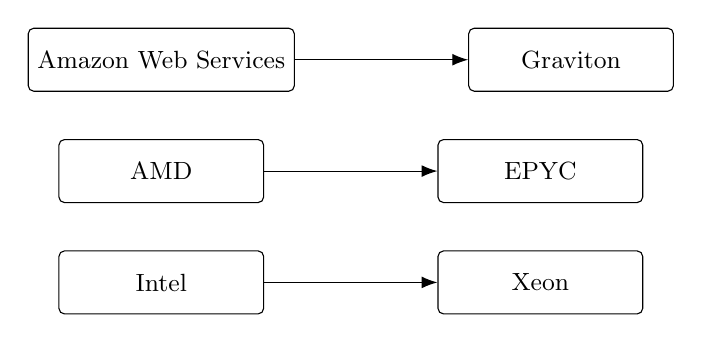
\begin{tikzpicture}[
  node distance=6mm,
  box/.style={draw, rounded corners=2pt, minimum height=8mm,
              minimum width=26mm, align=center, font=\small},
  arr/.style={-{Latex[length=2mm]}}
]
\node[box] (aws)   {Amazon Web Services};
\node[box, below=of aws] (amd)   {AMD};
\node[box, below=of amd] (intel) {Intel};

\node[box, right=22mm of aws]   (grav) {Graviton};
\node[box, right=22mm of amd]   (epyc) {EPYC};
\node[box, right=22mm of intel] (xeon) {Xeon};

\draw[arr] (aws)   -- (grav);
\draw[arr] (amd)   -- (epyc);
\draw[arr] (intel) -- (xeon);
\end{tikzpicture}
\end{center}

The three families differ at the instruction-set level (Graviton
implements ARM; EPYC and Xeon implement x86-64) and further in
microarchitecture, cache hierarchy, multicore organisation,
interconnect, and I/O design. The paper studies how these architectural
choices affect performance, scalability, and energy efficiency.

To keep the comparison tractable, the team has decided to focus on one
representative modern generation per family rather than every
generation ever released: \textbf{AWS Graviton4}, \textbf{AMD EPYC 9005
(Turin)}, and \textbf{Intel Xeon 6 (Granite Rapids)}. These three
generations were selected because comparative benchmark data exists for
all three running on the same cloud platform and instance
family~\cite{phoronix2025}, which reduces the confounding effect of
differing system configurations.
\subsection{Why the Topic was Selected}

The server processor landscape is undergoing a fundamental shift.  For
decades, x86 processors from Intel and AMD dominated data centres.  The
emergence of AWS Graviton — custom ARM-based silicon optimised for cloud
workloads — challenges the hegemony of x86 and raises deep architectural
questions about ISA efficiency, power-performance trade-offs, and vertical
integration.  This topic directly applies almost every major concept taught
in ELL305 (ISA design, pipelining, memory hierarchy, multiprocessors) to
real, commercially deployed hardware, making it both academically rigorous
and practically relevant.
\subsection{Mapping to the Prescribed Textbook}

\textbf{Textbook:} \textit{Basic Computer Architecture}, Smruti R.\ Sarangi,
Version~3.09, 2025.\\
\textbf{URL:} \url{https://srsarangi.github.io/archbook/archbook.pdf}

The chosen topic maps to several chapters of the prescribed textbook,
covering instruction-set design, ARM and x86 architectures, processor
design, pipelining, memory systems, and multiprocessor systems. The
specific chapters and their relevance to the proposed comparison are
summarised in Table~\ref{tab:textbook-map}. This mapping provides the
computer-architecture foundation required to analyse the architectural
differences among AWS Graviton, AMD EPYC, and Intel Xeon.

\begin{table}[h!]
\centering
\small
\renewcommand{\arraystretch}{1.35}
\begin{tabularx}{\linewidth}{>{\bfseries}l X}
\toprule
Chapter / Section & Relevance to the Term Paper \\
\midrule
Ch.\ 1, \S1.5 --- Instruction Set Design &
  RISC vs.\ CISC distinction; motivates the ARM64 (Graviton) vs.\
  x86-64 (EPYC, Xeon) comparison. \\
Ch.\ 4 --- ARM Assembly Language &
  ISA-level foundation for Graviton's ARM64 execution model,
  register file, and addressing modes. \\
Ch.\ 5 --- x86 Assembly Language &
  ISA-level foundation for EPYC and Xeon; CISC encoding, micro-op
  translation. \\
Ch.\ 9 --- Processor Design &
  Fetch/Decode/Execute/MA/RW pipeline stages; control unit; hardwired
  vs.\ microprogrammed design --- vocabulary for comparing all three chips. \\
Ch.\ 10 --- Principles of Pipelining &
  \S10.4 hazards, \S10.9 performance metrics (CPI, IPC),
  \S10.10 power/temperature (ED$^2$), \S10.11 branch prediction,
  multiple-issue, and out-of-order execution. \\
Ch.\ 11 --- The Memory System &
  \S11.2 caches, \S11.3 miss penalties, \S11.4 virtual memory and MMU
  --- used to compare L1/L2/L3 hierarchies, NUMA topology, and
  virtualisation support. \\
Ch.\ 12 --- Multiprocessor Systems &
  \S12.1 Moore's Law, \S12.4 MIMD/coherence/consistency,
  \S12.4.4 UMA vs.\ NUMA, \S12.6 interconnection networks
  (Infinity Fabric, Intel UPI, Graviton fabric). \\
Appendix~A --- Case Studies of Real Processors &
  AMD Bulldozer (\S A.2.2) and Intel Sandy Bridge (\S A.3.2) serve as
  the methodological template for our processor case-study chapters. \\
\bottomrule
\end{tabularx}
\caption{Textbook coverage map for the term paper.}
\label{tab:textbook-map}
\end{table}

\medskip
\noindent\textbf{Faculty consultation.} As this topic is drawn from
Chapters 1--12, the team will consult \textbf{Prof.\ Sumantra
DuttaRoy} for questions on the topic and its textbook mapping, per the
course rule that Chapters 1--12 route to Prof.\ DuttaRoy and Chapter 13
routes to Prof.\ Sarangi.

\subsection{Progress So Far (Gantt Chart)}

The chart below shows the work completed or currently in progress up to
\textbf{24 August 2026}. It is intended as a record of progress made so
far rather than a detailed plan for the future. The detailed schedule
for subsequent drafts and the final submission will be developed in
later drafts.

\noindent\textbf{Work-package breakdown}

\begin{itemize}[leftmargin=*, itemsep=2pt]

\item \textbf{WP1 -- Textbook Study.}
  \begin{itemize}[itemsep=1pt]
    \item Task 1: Read the basic chapters.
      \begin{itemize}[itemsep=1pt]
        \item Read Ch.~1 (Introduction), Ch.~4 (ARM ISA), and
        Ch.~5 (x86 ISA) --- \textbf{70\%} done by 24 Aug 2026.
        
        \item Read Ch.~9 (Processor Design) and Ch.~10 (Pipelining)
        --- \textbf{50\%} done.
        
        \item Read Ch.~11 (Memory System), Ch.~12 (Multiprocessors),
        and Appendix~A --- \textbf{30\%} done.
      \end{itemize}
      
    \item Task 2: Read papers related to the topic and store the
    references and PDFs in Zotero.
  \end{itemize}

\item \textbf{WP2 -- Literature.}
  \begin{itemize}[itemsep=1pt]
    \item Task 3: 9 references identified and collected so far
    (full list given in the following subsection).
  \end{itemize}
\begin{figure}[H]
    \centering

    \begin{ganttchart}[
        hgrid=false,
        vgrid,
        x unit=0.78cm,
        y unit chart=0.62cm,
        bar height=0.52,
        bar/.append style={
            fill=gray!30,
            draw=gray!60
        },
        bar label font=\scriptsize,
        title label font=\large\bfseries,
        title height=1,
        title/.append style={
            fill=white,
            draw=none
        },
        milestone label font=\scriptsize,
        milestone/.append style={
            fill=gray!35,
            draw=gray!60
        }
    ]{1}{12}

    % Month headings
    \gantttitle{}{1}
    \gantttitle{\textbf{Sep}}{4}
    \gantttitle{\textbf{Oct}}{4}
    \gantttitle{\textbf{Nov}}{3}
    \\

    % WP1 -- Textbook Study
    \ganttbar{WP1 -- Textbook Study}{1}{3} \\

    \ganttbar{Task 1a: Ch.\,1,4,5 (ISA)}{1}{1} \\

    \ganttbar{Task 1b: Ch.\,9,10 (Pipeline)}{1}{2} \\

    \ganttbar{Task 1c: Ch.\,11,12, App.\,A}{2}{3} \\

    \ganttbar{Task 2: Papers and Zotero}{1}{3} \\

    % WP2 -- Literature
    \ganttbar{WP2 -- Literature}{2}{6} \\

    \ganttbar{Task 3: References identified/read}{2}{6} \\

    % WP3 -- Draft Writing
    \ganttbar{WP3 -- Draft Writing}{4}{12} \\

    \ganttbar{Task 4: Draft 2 content}{4}{7} \\

    \ganttbar{Task 5: Draft 3 content}{7}{10} \\

    \ganttbar{Task 6: Benchmark data collection}{6}{10} \\

    \ganttbar{Task 7: Final synthesis}{10}{12} \\

    % Submission rows
    \ganttbar{Draft 2}{8}{8} \\

    \ganttbar{Draft 3 and Final}{10}{12}

    % 24 August reporting-date marker
    \ganttvrule[
        vrule/.append style={
            dashed,
            line width=0.9pt
        }
    ]{24 Aug 2026}{1}

\end{ganttchart}

\caption{Gantt chart showing the textbook study, literature collection,
draft writing, benchmarking, and final synthesis activities. The dashed
vertical line marks the reporting date of 24 August 2026.}
\label{fig:gantt}
\end{figure}

    \caption{Gantt chart showing the textbook study, literature collection,
    paper reading, drafting, benchmarking, and final synthesis activities.
    The dashed vertical line marks the current reporting date,
    24 August 2026.}
    \label{fig:gantt}
\end{figure}


\subsection{Preliminary Technical Understanding}
\label{sec:tech}

\subsubsection*{ISA Comparison: ARM64 vs.\ x86-64}
AWS Graviton implements the \textbf{ARMv8.x/ARMv9} ISA --- a
\emph{RISC} architecture with fixed 32-bit instruction width, 31
general-purpose registers, and a load/store-only memory model. EPYC and
Xeon implement \textbf{x86-64} --- a \emph{CISC} ISA with
variable-length encoding (1--15 bytes), 16 architectural registers, and
memory operands in arithmetic instructions. Xeon and EPYC both
translate x86 macro-ops into internal RISC-like micro-ops before the
out-of-order engine, adding a decode step absent in Graviton.

\subsubsection*{Microarchitecture of the Three Chosen Generations}
\begin{description}[leftmargin=2em, itemsep=3pt]
  \item[AWS Graviton4 (2024)] Neoverse~V2 core; 96 cores per socket;
        foundry/process node not publicly disclosed by AWS; SVE2 at a
        128-bit vector length (four 128-bit pipelines, \emph{not} 512-bit
        as sometimes assumed); 6-wide decode, 8-wide
        dispatch~\cite{chipsandcheese_graviton4}.
  \item[AMD EPYC 9005 ``Turin'' (2024)] Zen~5 (standard) or Zen~5c
        (dense) cores; up to 128 cores (Zen~5: 16 CCDs $\times$ 8 cores,
        TSMC 4\,nm) or up to 192 cores (Zen~5c: 12 CCDs $\times$ 16
        cores, TSMC 3\,nm), plus a separate I/O die; novel dual
        4-wide decode clusters, up to 8-wide combined with
        SMT~\cite{amdepyc,hothardware_turin,chipsandcheese_zen5}.
  \item[Intel Xeon 6900P ``Granite Rapids'' (2024)] Redwood~Cove
        P-core; up to 128 cores per socket; Intel~3 process; AMX
        (Advanced Matrix Extensions) support; front end inherited from
        Golden Cove's 6-wide decode~\cite{intelxeon,hothardware_xeon6}.
\end{description}
\subsubsection*{Pipeline Design and Out-of-Order Execution}
All three processors are deeply superscalar, out-of-order designs, each
built around Tomasulo-style reservation stations, a reorder buffer
(ROB) for precise exceptions, and aggressive branch prediction ---
concepts grounded in \S10.11 of the textbook.

\begin{figure}[h!]
\centering
\begin{tikzpicture}[
  stage/.style={draw=iitdblue, thick, fill=iitdblue!10,
                minimum width=2.15cm, minimum height=1.0cm, align=center, font=\small},
  arrow/.style={-{Latex[length=2mm]}, thick, iitdblue}
]
  \node[stage] (if) {Fetch\\(IF)};
  \node[stage, right=0.55cm of if] (id) {Decode\\(ID)};
  \node[stage, right=0.55cm of id] (ex) {Execute\\(EX)};
  \node[stage, right=0.55cm of ex] (ma) {Mem.\ Access\\(MA)};
  \node[stage, right=0.55cm of ma] (wb) {Write-back\\(RW)};
  \draw[arrow] (if) -- (id);
  \draw[arrow] (id) -- (ex);
  \draw[arrow] (ex) -- (ma);
  \draw[arrow] (ma) -- (wb);
  \node[below=0.5cm of ex, font=\footnotesize, align=center, text width=8cm]
    {Reservation stations + reorder buffer (ROB) sit around EX for
     out-of-order issue and precise exceptions (Graviton4, Zen~5, Redwood Cove).};
\end{tikzpicture}
\caption{Generic five-stage in-order front-end / out-of-order back-end
pipeline (Ch.~9--10) used as the reference model for comparing the three
processors.}
\label{fig:pipeline}
\end{figure}

\subsubsection*{Cache Hierarchy}
\begin{table}[h!]
\centering\small
\renewcommand{\arraystretch}{1.3}
\begin{tabular}{lccc}
\toprule
Level & Graviton4 & EPYC 9005 (Turin) & Xeon 6900P (Granite Rapids) \\
\midrule
L1-I & 64\,KB & 32\,KB & 32\,KB \\
L1-D & 64\,KB & 48\,KB & 48\,KB \\
L2   & 2\,MB  & 1\,MB  & 2\,MB  \\
L3 (shared, flagship SKU) & 36\,MB (96 cores) &
  up to 512\,MB (128 cores) & up to 504\,MB (128 cores) \\
\bottomrule
\end{tabular}
\caption{Cache hierarchy of the flagship SKU per family (per-core
unless noted). Sources:
Graviton4~\cite{chipsandcheese_graviton4}; EPYC~9005~\cite{amdepyc,hothardware_turin};
Xeon~6900P~\cite{intelxeon,hothardware_xeon6}.}
\label{tab:cache}
\end{table}

\subsubsection*{Multi-core and Multi-chip Interconnects}
\begin{itemize}[leftmargin=*, itemsep=2pt]
  \item \textbf{EPYC:} AMD Infinity Fabric --- die-to-die coherence
        across up to 16 CCDs; NUMA topology.
  \item \textbf{Xeon:} Intel UPI (Ultra Path Interconnect) for
        multi-socket; mesh-based on-die interconnect for tile
        coherence.
  \item \textbf{Graviton:} AWS proprietary on-package fabric;
        single-socket design targeting TCO over raw throughput.
\end{itemize}

\subsubsection*{Virtualisation}
All three support hardware virtualisation: ARM VHE/VHE+NV2, AMD-V with
SEV-SNP, and Intel VT-x with TDX. AWS's Nitro System additionally
offloads hypervisor functions to dedicated ASICs, reducing
virtualisation overhead in a way that is unique to Graviton-based
instances.
\subsection{References Read So Far}

\begin{itemize}[leftmargin=*, itemsep=2pt]
\item Sarangi~\cite{sarangi} --- prescribed textbook 
\item Velten et al.~\cite{velten2022} --- experimentally compares the
  memory hierarchy of AMD EPYC Rome and Intel Cascade Lake SP.
\item AWS~\cite{awsgravitonguide} --- official AWS Graviton technical
  guide (architecture, tooling, migration notes).
\item AMD~\cite{amdepyc} --- AMD EPYC 9005 (Turin) architecture
  overview, doc.\ 58462, Rev.\ 1.0.
\item Intel~\cite{intelxeon} --- Intel Xeon 6 architecture support
  article on performance and efficiency cores.
\item Larabel~\cite{phoronix2022} --- Phoronix same-cloud benchmark of
  Graviton/Graviton2/Graviton3 vs.\ EPYC Milan vs.\ Xeon Ice Lake
  (earlier generations; see the flag in Section~1.1).
\item Lawenda et al.~\cite{lawenda2025} --- effect of AMD EPYC L3
  cache size on CFD application performance.
\item Hofmann et al.~\cite{hofmann2015} --- Execution-Cache-Memory
  performance model for predicting memory-bound kernel performance.
\item AWS~\cite{awsperftesting} --- AWS whitepaper on Graviton
  performance-testing methodology for ISVs.
\end{itemize}
\clearpage
\bibliographystyle{unsrt}
\bibliography{refs}

\end{document}
